        \section{Convex Functionals}
We already had some different types of convexity, namely \hyperlink{definition_2_4_2}{Definition 2.4.2} and \hyperlink{definition_2_4_8}{Definition 2.4.8}. We also want to fix the most common notion in a more general setting.\\[11pt]

\textbf{\underline{Definition 3.2.1}}\\
(Convexity)\\
Let $X$ be a linear space.
\begin{itemize}
	\item[(i)] A set $M\subset X$ is called \textit{convex} if for all $x,y\in M$ and all $\lambda\in(0,1)$ we have $(1-\lambda)x+\lambda y\in M$.
	\item[(ii)] A mapping $I:X\longrightarrow\mathbb{R}_\infty$ is called \textit{convex} if for all $x,y\in X$ and all $\lambda\in(0,1)$ it holds $I((1-\lambda)x+\lambda y)\leq(1-\lambda)I(x)+\lambda I(y)$.\\[11pt]
\end{itemize}

\hypertarget{remark_3_2_2}{\textbf{Remark 3.2.2}}\\
A functional $I:X\longrightarrow\mathbb{R}_\infty$ is convex if and only if the epigraph $\epi{I}$ is convex. Furthermore, $I$ is convex if and only if all the sublevel sets $S_\alpha(I)$ for $\alpha\in\mathbb{R}$ are convex.\\[11pt]

\textbf{Examples 3.2.3}
\begin{itemize}
	\item[(a)] For a normed space $X$ and any $p\geq1$, the functional $I:X\longrightarrow\mathbb{R}$, $I(x)=\lVert x\rVert_X^p$ is convex. (This is because $I$ is the composition of the norm $X\longrightarrow[0,\infty)$, $u\longmapsto\lVert u\rVert_X$ (which is convex by triangular inequality) and the mapping $[0,\infty)\longrightarrow[0,\infty)$, $c\longmapsto c^p$ (which is convex and monotonically increasing for all $p\geq1$).)

	\begin{figure}[ht]
		\centering
		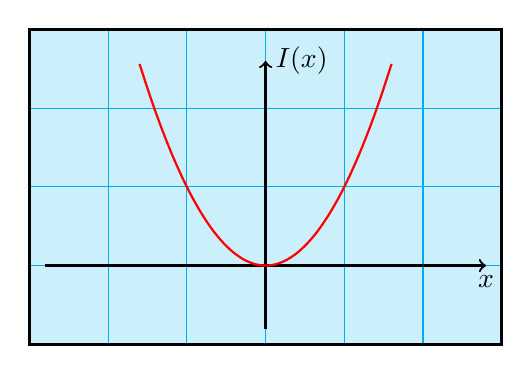
\begin{tikzpicture}
			% Hintergrund und Achsen
			\fill[cyan!20] (-3, -1) rectangle (3, 3);
			\draw[cyan] (-3, -1) grid (3, 3);
			\draw[thick, ->] (-2.8, 0) -- (2.8, 0) node[below] {$x$};
			\draw[thick, ->] (0, -0.8) -- (0, 2.6) node[right] {$I(x)$};
			\draw[very thick] (-3, -1) rectangle (3, 3);

			% Funktion
			\draw[thick, red] plot[smooth, domain=-1.6:1.6] (\x, {(\x)^2});
		\end{tikzpicture}
		\caption{Illustration for $(X,\lVert\cdot\rVert_X)=(\mathbb{R},\lvert\cdot\rvert)$ and $p=2$.}
	\end{figure}
	\item[(b)] For a set $M\subset X$ we define the so-called \textit{indicator function}

	\begin{figure}[ht]
		\centering
		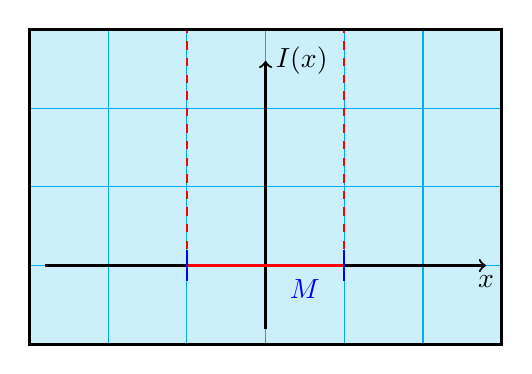
\begin{tikzpicture}
			% Hintergrund und Achsen
			\fill[cyan!20] (-3, -1) rectangle (3, 3);
			\draw[cyan] (-3, -1) grid (3, 3);
			\draw[thick, ->] (-2.8, 0) -- (2.8, 0) node[below] {$x$};
			\draw[thick, ->] (0, -0.8) -- (0, 2.6) node[right] {$I(x)$};

			% Funktion
			\draw[thick, red] (-1, 0) -- (1, 0);
			\draw[thick, red, dashed] (-1, 0) -- (-1, 3);
			\draw[thick, red, dashed] (1, 0) -- (1, 3);

			% Menge M
			\draw[thick, blue] (-1, 0.2) -- (-1, -0.2);
			\draw[thick, blue] (1, 0.2) -- (1, -0.2);
			\node[blue] at (0.5, -0.3) {$M$};

			\draw[very thick] (-3, -1) rectangle (3, 3);
		\end{tikzpicture}
		\caption{Illustration for $(X,\lVert\cdot\rVert_X)=(\mathbb{R},\lvert\cdot\rvert)$ and $M=[-1,1]$.}
	\end{figure}

	\[I(x)=\chi_M(x)=\left\{\begin{array}{rl}
		0&\text{for }x\in M,\\
		\infty&\text{for }x\notin M.
	\end{array}\right.\]

	One can easily show that $I$ is convex if and only if $M$ is convex.
	\item[(c)] For a convex set $M$, $I(x)=\lVert x\rVert_X^p+\chi_M(x)$ is convex.

	\begin{figure}[ht]
		\centering
		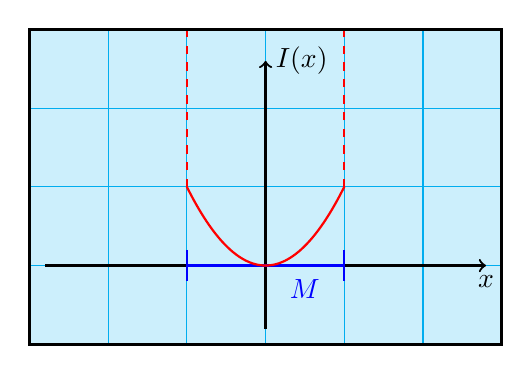
\begin{tikzpicture}
			% Hintergrund und Achsen
			\fill[cyan!20] (-3, -1) rectangle (3, 3);
			\draw[cyan] (-3, -1) grid (3, 3);
			\draw[thick, ->] (-2.8, 0) -- (2.8, 0) node[below] {$x$};
			\draw[thick, ->] (0, -0.8) -- (0, 2.6) node[right] {$I(x)$};

			% Menge M
			\draw[thick, blue] (-1, 0.2) -- (-1, -0.2);
			\draw[thick, blue] (1, 0.2) -- (1, -0.2);
			\draw[thick, blue] (-1, 0) -- (1, 0);
			\node[blue] at (0.5, -0.3) {$M$};

			% Funktion
			\draw[thick, red] plot[smooth, domain=-1:1] (\x, {(\x)^2});
			\draw[thick, red, dashed] (-1, 1) -- (-1, 3);
			\draw[thick, red, dashed] (1, 1) -- (1, 3);

			\draw[very thick] (-3, -1) rectangle (3, 3);
		\end{tikzpicture}
		\caption{Illustration for $(X,\lVert\cdot\rVert_X)=(\mathbb{R},\lvert\cdot\rvert)$, $p=2$ and $M=[-1,1]$.}
	\end{figure}

	More general, the sum of two convex functions again is convex.\\[11pt]
\end{itemize}

\hypertarget{theorem_3_2_4}{\textbf{\underline{Theorem 3.2.4}}}\\
(Hahn-Banach separation theorem)\\
Let $X$ be a Banach space, and let $A,B\subset X$ be non-empty, convex sets with $A\cap B=\emptyset$.
\begin{itemize}
	\item[(i)] If $A$ is open, then there exists $\varphi\in X'$ such that $\varphi(a)<\varphi(b)$ for all $a\in A$, $b\in B$.
	\item[(ii)] If $A$ is closed and $B$ compact, then there exist $\varphi\in X'$ and $\alpha,\beta\in\mathbb{R}$ such that for all $a\in A$, $b\in B$ it holds $\varphi(a)\leq\alpha<\beta\leq\varphi(b)$.\\
\end{itemize}

\textit{Proof:}\\
This is done in course \textit{Functional Analysis}.\hfill$\blacksquare$\\[11pt]

\hypertarget{lemma_3_2_5}{\textbf{Lemma 3.2.5}}\\
(Mazur's lemma)\\
Let $X$ be a Banach space and $M\subset X$ convex. Then $M$ is strongly sequentially closed if and only if $M$ is weakly sequentially closed.\\

\textit{Proof:}
\begin{itemize}
	\item[($\Rightarrow$)] Consider $(u_n)_{n\in\mathbb{N}}\subset M$, $u\in X$ with $u_n\rightharpoonup u$ in $X$ as $n\to\infty$. We need to see $u\in M$. Assume that $u\notin M$. Choose $A=M$ and $B=\{u\}$. Then $A$, $B$ are both clearly non-empty, convex, and by assumption $u\notin M=A$, so $A\cap B=\emptyset$. Moreover, $A$ is strongly sequentially closed, i.e. closed. Thus, \hyperlink{theorem_3_2_4}{Theorem 3.2.4 (ii)} yields $\varphi\in X'$, $\alpha,\beta\in\mathbb{R}$ with $\varphi(a)\leq\alpha<\beta\leq\varphi(u)$ for all $a\in A$. But $u_n\rightharpoonup u$ for $n\to\infty$, so in particular
	\[\varphi(u)=\lim_{n\to\infty}{\varphi(u_n)}\leq\alpha<\beta\leq\varphi(u)\]
	which is a contradiction. Hence, $u\in M$.
	\item[($\Leftarrow$)] This is clear because any strongly convergent sequence also converges weakly to the same limit.\hfill$\blacksquare$\\[11pt]
\end{itemize}

\hypertarget{theorem_3_2_6}{\textbf{\underline{Theorem 3.2.6}}}\\
Let $X$ be a Banach space and let $I:X\longrightarrow\mathbb{R}_\infty$ be convex and lower semicontinuous. Then $I$ is weakly lower semicontinuous.\\

\textit{Proof:}\\
Since $I$ is convex, all sublevel sets $S_\alpha(I)$ for $\alpha\in\mathbb{R}$ are convex by \hyperlink{remark_3_2_2}{Remark 3.2.2}. And since $I$ is lower semicontinuous, all $S_\alpha(I)$ are (strongly) closed by \hyperlink{theorem_3_1_15}{Theorem 3.1.15}. By \hyperlink{lemma_3_2_5}{Lemma 3.2.5}, i.e. Mazur's lemma, all $S_\alpha(I)$ are therefore weakly closed. Hence, \hyperlink{theorem_3_1_15}{Theorem 3.1.15} tells us that $I$ is weakly lower semicontinuous.\hfill$\blacksquare$\\[11pt]

\hypertarget{corollary_3_2_7}{\textbf{Corollary 3.2.7}}\\
(Abstract existence theorem for convex functionals)\\
Let $X$ be a reflexive Banach space. Let $I:X\longrightarrow\mathbb{R}_\infty$ be coercive, convex and lower semicontinuous. Then the direct problem has a solution, i.e. there exists $u_*\in X$ such that $I(u_*)=\inf\{I(v)\mid v\in X\}$.\\

\textit{Proof:}\\
Combine the abstract existence theorem, \hyperlink{theorem_3_1_14}{Theorem 3.1.14}, with \hyperlink{theorem_3_2_6}{Theorem 3.2.6}.\hfill$\blacksquare$\\[11pt]

Previously, we investigated minimizers via critical points for which we needed some differentiability condition. In our abstract existence results such restrictive regularity assumptions on $I$ are no longer needed. So we have an existence result for a huge class of special convex functionals. To further investigate minimizers, we need a good notion of derivative for convex functionals.\\

\textbf{\underline{Definition 3.2.8}}\\
(Subdifferential)\\
Let $X$ be a Banach space, $I:X\longrightarrow\mathbb{R}_\infty$ a functional. Let $u\in X$.
\begin{itemize}
	\item[(i)] A functional $\varphi\in X'$ is called a \textit{subgradient of $I$ in $u$} if for all $v\in X$
	\[I(v)\geq I(u)+\varphi(v-u).\]
	\item[(ii)] The set $\partial I(u)=\{\varphi\in X'\mid\varphi\text{ is a subgradient of }I\text{ in }u\}$ is called the \textit{subdifferential of $I$ in $u$}.\\
\end{itemize}

To get a feeling for subdifferentials, one can think of the right-hand side ``$I(u)+\varphi(v-u)$'' as an affine function in $v$, like a tangential plane or a Taylor expansion of first order which always has to be below $I$. We will discuss some examples.\\[11pt]

\hypertarget{remark_3_2_9}{\textbf{Remark 3.2.9}}
\begin{itemize}
	\item[(a)] It is possible that $\partial I(u)=\emptyset$ for some $u\in X$, so this is allowed.
	\item[(b)] If $I\not\equiv+\infty$ and $\partial I(u)\ne\emptyset$ for some $u\in X$, then $I(u)<\infty$. Indeed, if $\varphi\in\partial I(u)$, then, if $v\in X$ satisfies $I(v)<\infty$, we obtain $\infty>I(v)-\varphi(v-u)\geq I(u)$.\\[11pt]
\end{itemize}

\textbf{Example 3.2.10}\\
(Modulus functional)\\
Consider $I:\mathbb{R}\longrightarrow\mathbb{R}$, $I(x):=\lvert x\rvert$. To compute the subdifferential, we have to ask what kind of affine function lies below $I$.

\begin{figure}[ht]
	\centering
	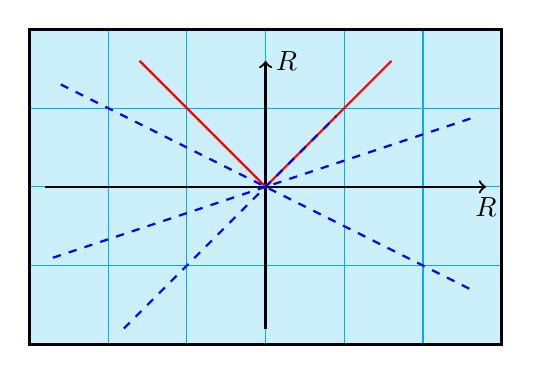
\begin{tikzpicture}
		% Hintergrund und Achsen
		\fill[cyan!20] (-3, -2) rectangle (3, 2);
		\draw[cyan] (-3, -2) grid (3, 2);
		\draw[thick, ->] (-2.8, 0) -- (2.8, 0) node[below] {$\mathbb{R}$};
		\draw[thick, ->] (0, -1.8) -- (0, 1.6) node[right] {$\mathbb{R}$};
		\draw[very thick] (-3, -2) rectangle (3, 2);

		% Funktionen
		\draw[thick, red] (-1.6, 1.6) -- (0, 0) -- (1.6, 1.6);
		\draw[thick, blue, dashed] (-1.8, -1.8) -- (0.9, 0.9);
		\draw[thick, blue, dashed] (-2.6, 1.3) -- (2.6, -1.3);
		\draw[thick, blue, dashed] (-2.7, -0.9) -- (2.7, 0.9);
	\end{tikzpicture}
	\caption{Graph of modulus functional (red) and some subdifferentials in 0 (blue).}
\end{figure}

We obtain
\[\partial I(x)=\left\{\begin{array}{rl}
	1&\text{if }x>0,\\
	{[-1,1]}&\text{if }x=0,\\
	-1&\text{if }x<0.
\end{array}\right.\]\\

\textbf{Example 3.2.11}\\
(Indicator function)\\
Let $\emptyset\ne M\subset X$ and consider
\[\chi_M:X\longrightarrow\mathbb{R}_\infty,\qquad\chi_M(x):=\left\{\begin{array}{rl}
	0&\text{if }u\in M,\\
	+\infty&\text{if }u\notin M.
\end{array}\right.\]
If $u\notin M$, we clearly have $\partial\chi_M(u)=\emptyset$ by \hyperlink{remark_3_2_9}{Remark 3.2.9 (b)}. If $u\in M$, then $\varphi\in\partial\chi_M(u)$ if and only if $I(v)\geq I(u)+\varphi(v-u)$ for all $v\in X$. This is equivalent to $0\geq\varphi(v-u)$ for all $v\in M$ (since $I(v)=I(u)=0$ for $v\in M$).\\

For $u\in\interior{M}$, we have $B_{\varepsilon_0}(u)\subset M$ for some suitable $\varepsilon_0>0$. Choose $v=u+\varepsilon h$ for $0<\varepsilon<\varepsilon_0$ and $h\in X$ with $\lVert h\rVert_X=1$. Then
\[0\geq\varphi(v-u)=\varphi(\varepsilon h)=\varepsilon\varphi(h),\]
i.e. $0\geq\varphi(h)$ for all $h\in X$ with $\lVert h\rVert_X=1$. Repeat the argument with $\tilde{h}=-h$ to get $0\leq\varphi(h)$. Thus, $0=\varphi(h)$ for all $h\in X$ with $\lVert h\rVert_X=1$. As a consequence $\lVert\varphi\rVert_{X'}=0$, i.e. $\varphi=0$. Altogether we see
\[\partial\chi_M(u)=\left\{\begin{array}{rl}
	\emptyset&\text{if }u\notin M,\\
	\{0\}&\text{if }u\in\interior{M},\\
	\{\varphi\in X'\mid\varphi(u)\geq\varphi(v)\text{ for all }v\in M\}&\text{if }u\in M.
\end{array}\right.\]\\

As an example, take $X=\mathbb{R}$ and $M=[0,\infty)$. Then
\[\partial\chi_M(u)=\left\{\begin{array}{rl}
	\emptyset&\text{if }u<0,\\
	\{0\}&\text{if }u>0,\\
	(-\infty,0]&\text{if }u=0
\end{array}\right.\]
since for $u=0$ we have $\varphi(v)\leq\varphi(u)=0$ for all $v\in[0,\infty)$, so, if $\varphi(x)=ax$ for some $a\in\mathbb{R}$, then $a\leq0$.\\

\begin{figure}[ht]
	\centering
	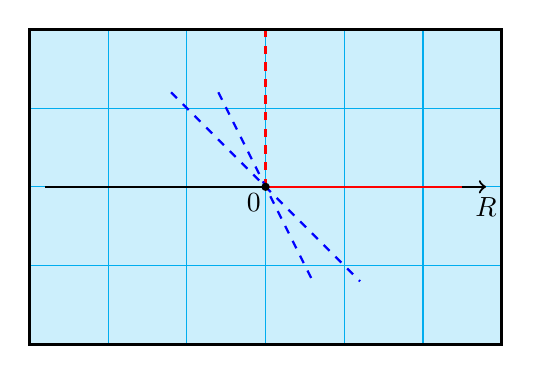
\begin{tikzpicture}
		% Hintergrund und Achsen
		\fill[cyan!20] (-3, -2) rectangle (3, 2);
		\draw[cyan] (-3, -2) grid (3, 2);
		\draw[thick, ->] (-2.8, 0) -- (2.8, 0) node[below] {$\mathbb{R}$};

		% Funktionen
		\draw[thick, red] (0, 0) -- (2.5, 0);
		\draw[thick, red, dashed] (0, 0) -- (0, 2);
		\draw[thick, blue, dashed] (-1.2, 1.2) -- (1.2, -1.2);
		\draw[thick, blue, dashed] (-0.6, 1.2) -- (0.6, -1.2);
		\fill circle (1.5pt);
		\node at (-0.15, -0.2) {0};

		\draw[very thick] (-3, -2) rectangle (3, 2);
	\end{tikzpicture}
	\caption{Graph of indicator function (red) and some subdifferentials in 0 (blue).}
\end{figure}
\leavevmode\\[11pt]

\textbf{Proposition 3.2.12}\\
(Global minimizers and subdifferentials)\\
Let $X$ be a Banach space, not necessarily reflexive, $I:X\longrightarrow\mathbb{R}_\infty$ a functional and $u_*\in X$. Then $I(u_*)=\inf\{I(u)\mid u\in X\}$ if and only if $0\in\partial I(u_*)$.\\

\textit{Proof:}
\begin{align*}
	I(u_*)=\inf\{I(u)\mid u\in X\}\quad&\Longleftrightarrow\quad I(v)\geq I(u)\text{ for all }v\in X\\
	&\Longleftrightarrow\quad I(v)\geq I(u_*)+0(v-u)\text{ for all }v\in X\\
	&\Longleftrightarrow\quad0\in\partial I(u_*).
\end{align*}
\hfill$\blacksquare$\\[11pt]

How are subdifferentials related to classical derivative? For that, we introduce a new type of differentiability.\\

\textbf{\underline{Definition 3.2.13}}\\
(G\^ateaux derivative)\\
A functional $I:X\longrightarrow\mathbb{R}_\infty$ is called \textit{G\^ateaux differentiable in $u\in X$} with $I(u)<\infty$ if there exists $\varphi_u\in X'$ with
\[\lim_{t\to0}{\frac{1}{t}(I(u+th)-I(u))}=\varphi_u(h)\]
for all $h\in X$. In this case, we write $DI(u):=\varphi_u$ and this is called the \textit{G\^ateaux derivative of $I$ in $u$}.\\[11pt]

The G\^ateaux derivative is strongly related to the notion of the first variation. Indeed, $I$ is G\^ateaux differentiable if and only if the first variation exists and defines a linear continuous functional.\\[11pt]

\textbf{Proposition 3.2.14}\\
Let $X$ be a Banach space, $I:X\longrightarrow\mathbb{R}_\infty$ convex. Let $u\in X$ with $I(u)<\infty$. If $I$ is G\^ateaux differentiable in $u$ then $\partial I(u)=\{DI(u)\}$.\\

\textit{Remark: The subdifferential is a global concept, while G\^ateaux differentiability is local. Therefore we need $I$ to be convex.}\\

\textit{Proof:}\\
First we are going to show $DI(u)\in\partial I(u)$. For this, let $v\in X$ and define $\gamma(t)=I(u+t(v-u))$. Then $\gamma$ is convex since $I$ is, so
\[I(v)=\gamma(1)\geq\gamma(0)+\gamma'(0)(1-0)=I(u)+DI(u)[v-u],\]
therefore $DI(u)\in\partial I(u)$. Now show that $\partial I(u)\subset\{DI(u)\}$. Let $\varphi\in\partial I(u)$. For $h\in X$, $t\in\mathbb{R}$, we have $I(u+th)-I(u)\geq\varphi(th)$ (remind that $I(u)<\infty$). Therefore
\[DI(u)[h]=\lim_{t\nearrow0}{\frac{I(u+th)-I(u)}{t}}\leq\varphi(h)\leq\lim_{t\searrow0}{\frac{I(u+th)-I(u)}{t}}=DI(u)[h],\]
i.e. $DI(u)[h]=\varphi(h)$, i.e. $\varphi=DI(u)$, i.e. $\varphi\in\{DI(u)\}$.\hfill$\blacksquare$\\[11pt]

When is $I$ subdifferentiable? This means, when is $\partial I(u)\ne\emptyset$? We are interested in an answer for more general functionals.\\[11pt]

\hypertarget{theorem_3_2_15}{\textbf{\underline{Theorem 3.2.15}}}\\
Let $X$ be a Banach space, $I:X\longrightarrow\mathbb{R}_\infty$ convex. If $I$ is finite and continuous in $u\in X$, then $\partial I(u)\ne\emptyset$.\\

For the proof we need a lemma first.\\

\hypertarget{lemma_3_2_16}{\textbf{Lemma 3.2.16}}\\
Let $I:X\longrightarrow\mathbb{R}_\infty$ be convex, $I$ finite and continuous in $u\in X$. Then $(u,I(u)+1)\in\interior{\epi{I}}$.\\

\textit{Proof:}\\
If $I$ is continuous in $u$, then there exists $\delta_0>0$ such that for all $v\in X$ with $\lVert u-v\rVert_X<\delta_0$ we have $\lvert I(u)-I(v)\rvert\leq\frac{1}{2}$. In particular, for all $\alpha\in B_{1/2}(I(u)+1)$ and $v\in B_{\delta_0}(u)$ it holds $I(v)\leq\alpha$. Hence,
\[B_{\delta_0}(u)\times B_{1/2}(I(u)+1)\subset\epi{I}\subset X\times\mathbb{R},\]
so $(u,I(u)+1)\in\interior{\epi{I}}$.\hfill$\blacksquare$\\[11pt]

\textit{Proof of \hyperlink{theorem_3_2_15}{Theorem 3.2.15}:}\\
\hyperlink{lemma_3_2_16}{Lemma 3.2.16} implies $B:=\interior{\epi{I}}\ne\emptyset$. Since $I$ is convex, also $\epi{I}$ is convex, so $B$ is convex. Moreover, let $A:=\{(u,I(u))\}$ and apply Hahn-Banach separation theorem, i.e. \hyperlink{theorem_3_2_4}{Theorem 3.2.4 (i)}. Then there exists $\phi\in(X\times\mathbb{R})'\simeq X'\times\mathbb{R}$ such that $\phi(u,I(u))<\phi(v,\alpha)$ for all $(v,\alpha)\in B$.\\

We can write $\phi(v,\alpha)=\varphi(v)+\beta\alpha$ for some $\varphi\in X'$ and $\beta\in\mathbb{R}$. Choose $(u,I(u)+1)\in\interior{\epi{I}}$. Then
\[\varphi(u)+\beta I(u)<\varphi(u)+\beta(I(u)+1),\]
so $\beta>0$. Let $v\in X$ with $I(v)<\infty$. Then $(v,I(v))\in\epi{I}$. Since $\epi{I}$ is convex and $\interior{\epi{I}}\ne\emptyset$, we have that $\epi{I}\subset\overline{\interior{\epi{I}}}$ and hence we obtain
\[\varphi(u)+\beta I(u)\leq\varphi(v)+\beta I(v),\]
i.e. $I(u)\leq I(v)-\frac{1}{\beta}\varphi(u-v)$. But this also holds true if $I(v)=\infty$, whence $-\frac{1}{\beta}\varphi\in\partial I(u)$.\hfill$\blacksquare$\\[11pt]

\textbf{Proposition 3.2.17}\\
(Subdifferential calculus)\\
Let $X$ be a Banach space.
\begin{itemize}
	\item[(a)] If $I:X\longrightarrow\mathbb{R}_\infty$ is a functional and $\alpha>0$, then $\partial(\alpha I)(u)=\alpha\partial I(u)$ for all $u\in X$.
	\item[(b)] For two functionals $I_1,I_2:X\longrightarrow\mathbb{R}_\infty$ and $u\in X$ it holds
	\[\partial(I_1+I_2)(u)\supset\partial I_1(u)+\partial I_2(u).\]
	Equality holds if in addition
	\begin{itemize}
		\item[(i)] $I_1$, $I_2$ are both convex,
		\item[(ii)] $I_1(u_0),I_2(u_0)<\infty$ and $I_i$ is continuous in $u_0$ for some $u_0\in X$ and some $i\in\{1,2\}$.\\
	\end{itemize}
\end{itemize}

\textit{Proof:}
\begin{itemize}
	\item[(a)] We have
	\begin{align*}
		\varphi\in\partial(\alpha I)(u)\quad&\Longleftrightarrow\quad\alpha I(v)\geq\alpha I(u)+\varphi(v-u)\text{ for all }v\in X,\\
		&\Longleftrightarrow\quad I(v)\geq I(u)+\frac{1}{\alpha}\varphi(v-u)\\
		&\Longleftrightarrow\quad\frac{1}{\alpha}\varphi\in\partial I(u).
	\end{align*}
	\item[(b)] Let $\varphi_1\in\partial I_1(u)$ and $\varphi_2\in\partial I_2(u)$. Then for all $v\in X$
	\begin{align*}
		(I_1+I_2)(v)&=I_1(v)+I_2(v)\\
		&\geq I_1(u)+\varphi_1(v-u)+I_2(u)+\varphi_2(v-u),\\
		&=(I_1+I_2)(u)+(\varphi_1+\varphi_2)(v-u),
	\end{align*}
	whence $\varphi_1+\varphi_2\in\partial(I_1+I_2)(u)$.\\

	Now we assume the additional assumptions (i) and (ii) and let $\varphi\in\partial(I_1+I_2)(u)$. We need a functional in one of the subdifferentials $\partial I_1(u)$ or $\partial I_2(u)$ to work with. To this end, we will apply Hahn-Banach separation theorem in an appropriate way. First note that $I_1(u)<\infty$ for $i=1,2$ because $I_1+I_2\not\equiv\infty$. Without loss of generality we may assume that $I_1$ is continuous in $u_0$. Define
	\[G_u:X\longrightarrow\mathbb{R}_\infty,\qquad G_u(v):=I_1(v)-I_1(u)-\varphi(v-u).\]
	Then $G_u(v)\geq I_2(u)-I_2(v)$ for all $v\in X$. Moreover, we define
	\begin{align*}
		A&:=\epi{G_u}=\{(v,\alpha)\in X\times\mathbb{R}\mid G_u(v)\leq\alpha\},\\
		B&:=\{(w,\beta)\in X\times\mathbb{R}\mid\beta\leq I_2(u)-I_2(w)\}.
	\end{align*}
	Then $A$ and $B$ are convex because $I_1,I_2$ are convex. By hypothesis (ii) and \hyperlink{lemma_3_2_16}{Lemma 3.2.16} it holds $\interior{A}\ne\emptyset$. Furthermore, $\interior{A}\cap B=\emptyset$. Hence, Hahn-Banach separation theorem yields $(\tilde{\varphi},\gamma)\in X'\times\mathbb{R}$ such that $\tilde{\varphi}(w)+\gamma\beta<\tilde{\varphi}(v)+\gamma\alpha$ for all $(w,\beta)\in B$, $(v,\alpha)\in\interior{A}$, i.e. $\tilde{\varphi}(w)+\gamma\beta\leq\tilde{\varphi}(v)+\gamma\alpha$ for all $(w,\beta)\in B$, $(v,\alpha)\in A$.\\

	\textit{Claim:} $\gamma>0$.
	\begin{itemize}
		\item[] \hyperlink{lemma_3_2_16}{Lemma 3.2.16} and (ii) imply $(u_0,G_u(u_0)+1)\in\interior{\epi{G_u}}=\interior{A}$. Moreover, $(u_0,I_2(u)-I_2(u_0))\in B$. Then
		\[\tilde{\varphi}(u_0)+\gamma(I_2(u)-I_2(u_0))<\tilde{\varphi}(u_0)+\gamma(G_u(u_0)+1),\]
		so rearranging terms gives
		\[\gamma(\underbrace{I_2(u)-I_2(u_0)-G_u(u_0)}_{\leq0}-1)<0,\]
		so $\gamma>0$ as claimed.
	\end{itemize}

	Moreover, $(u,0)\in A\cap B$. Thus,
	\[\tilde{\varphi}(w)+\gamma\beta\leq\tilde{\varphi}(u)+\gamma\cdot0\leq\tilde{\varphi}(v)+\gamma\alpha\]
	for all $(w,\beta)\in B$, $(v,\alpha)\in A$. Using $(v,G_u(v))\in A$ and $(w,I_2(u)-I_2(w))\in B$ for $w,v\in X$ with $I_1(v),I_2(w)<\infty$, we obtain
	\[\tilde{\varphi}(w)+\gamma(I_2(u)-I_2(w))\leq\tilde{\varphi}(u)\leq\tilde{\varphi}(v)+\gamma G_u(v),\]
	hence $I_2(w)\geq I_2(u)+\frac{1}{\gamma}\tilde{\varphi}(w-u)$ and $I_1(v)\geq I_1(u)+\varphi(v-u)-\frac{1}{\gamma}\tilde{\varphi}(v-u)$. But these estimates hold also true for $I_1(v)=\infty$ and $I_2(w)=\infty$. We infer $\frac{1}{\gamma}\tilde{\varphi}\in\partial I_2(u)$ and $\varphi-\frac{1}{\gamma}\tilde{\varphi}\in\partial I_1(u)$. So
	\[\varphi=\left(\varphi-\frac{1}{\gamma}\tilde{\varphi}\right)+\frac{1}{\gamma}\tilde{\varphi}\in\partial I_1(u)+\partial I_2(u).\]
\end{itemize}
\hfill$\blacksquare$